
\chapter{WISDEM Floating Turbine Analysis}
\label{sec:other}
Direct WISDEM dependencies to \textit{CommonSE} and \textit{TowerSE}, as well as some of the
supporting utilities housed under the WISDEM umbrella, were mentioned in
Section \ref{sec:package}.  There are other inputs into \textit{FloatingSE} that
are outputs of other WISDEM modules.  For example force, moment, and
mass properties of the RNA.  An OpenMDAO Group that links these other
modules together to form a virtual floating turbine does not explicitly
fit within the conceptual boundaries of the \texttt{src/floatingse} package.
However, two other files within the \textit{FloatingSE} \texttt{src}-directory
(but outside the \texttt{src/floatingse} package) do assemble the virtual
floating turbine Group,

{\small
\begin{tabularx}{\linewidth}{ l X }
\texttt{floating\_turbine\_assembly.py} & OpenMDAO Group that connects  multiple WISDEM modules for a complete floating offshore turbine simulation and optimization.\\
\texttt{floating\_turbine\_instance.py} & Example implementing the above Group.
\end{tabularx}
}

\begin{figure}
  \begin{center}
    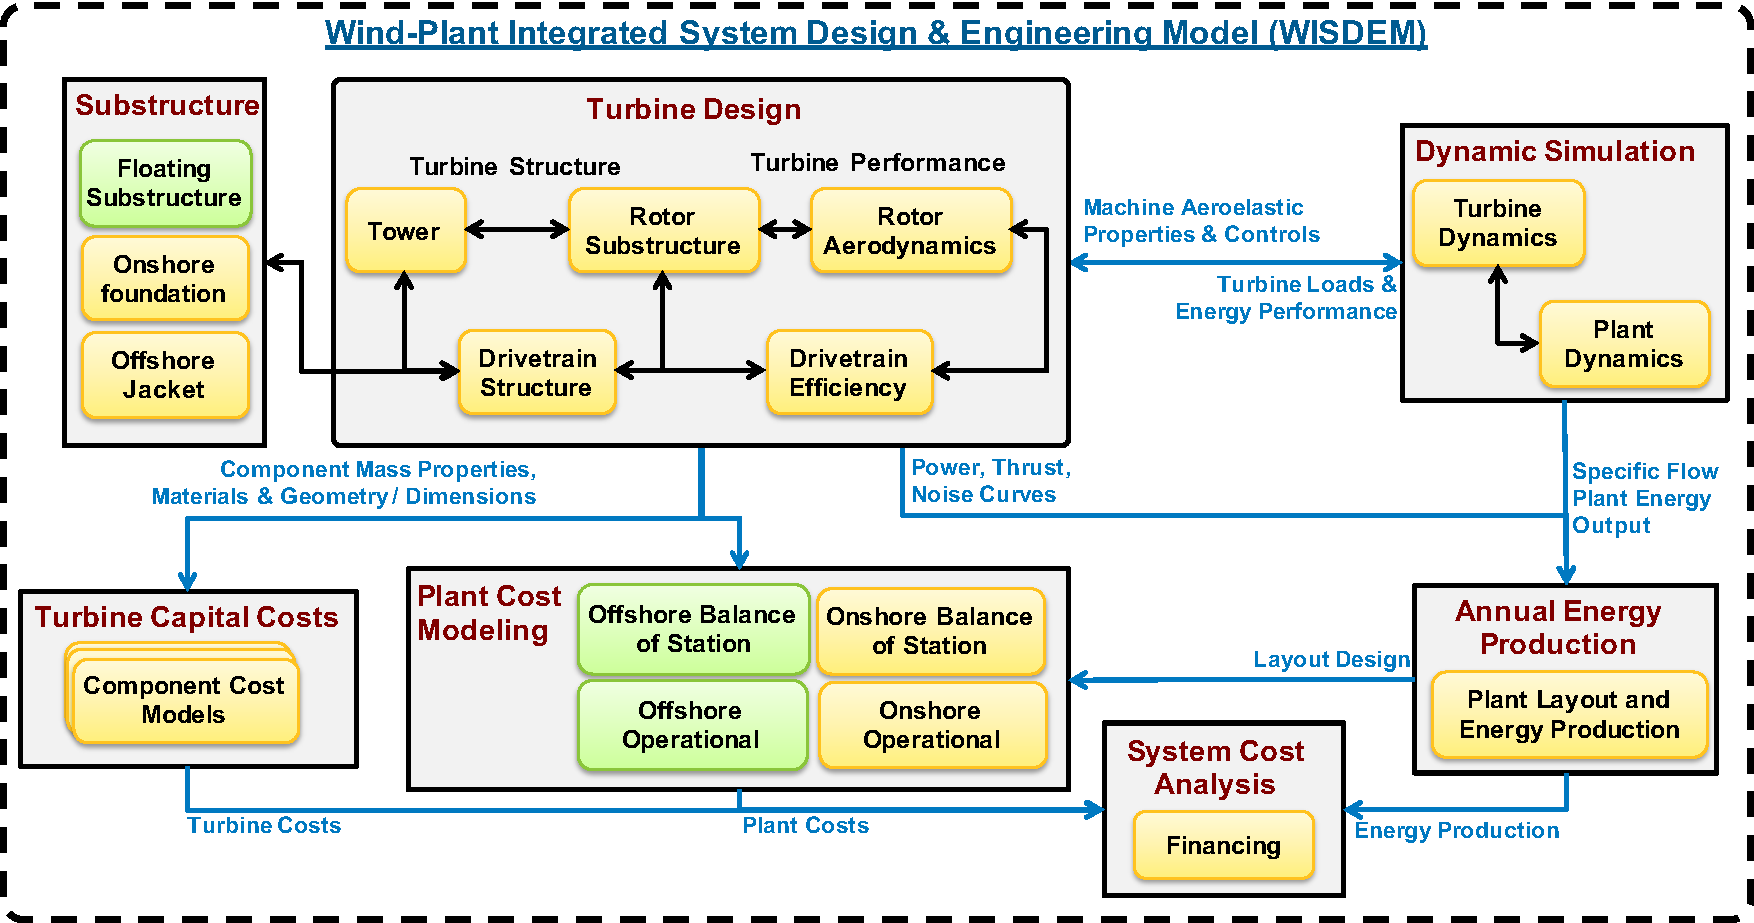
\includegraphics[width=6in]{figs/new_wisdem.pdf}
    \caption{Conceptual diagram of WISDEM following the addition of
      \textit{FloatingSE} and other modules to support offshore floating
      wind turbines.}
    \label{fig:new_wisdem}
  \end{center}
\end{figure}

The WISDEM modules that exchange inputs and outputs within this
high-level assembly are listed below, as well as the features that are
of interest to the virtual floating turbine simulation.
\begin{description}
\item[RotorSE]: Analysis of aerodynamic and structural loading of rotor
  blades, determination of turbine power curve, and calculation of
  annual energy production (AEP).
\item[CommonSE]: Wind and wave velocity profiles, drag calculations,
  probabilities distributions, frustum and tubular mass properties, math
  utilities, structural code compliance checks, and RNA aggregator.
\item[OffshoreBOS\_SE]: Capital costs for wind plant items aside from the
  turbine, such as cabling and substations.  Assembly, installation,
  commissioning, decommissioning, and financing costs for all
  components. See \citep{obos}.
\item[FloatingSE]: Floating substructure, including mooring and anchors, and
  static stability calculations.
\item[TurbineCostsSE (2015)]: Capital costs for all turbine components
  above the water line.
\item[PlantFinanceSE]: Roll-up of capital costs, balance of station
  costs, operational costs, financing rates, and net energy production
  into the levelized cost of energy (LCOE).
\item[DriveSE]: Analysis of drive shaft, bearings, and gearbox.  See
  \citep{DriveSE}. NOT YET IMPLEMENTED.
\item[Offshore\_OandM\_SE]: Operational and maintenance costs.  NOT YET
    DEVELOPED.
\end{description}
Note that as of this writing, two modules are not yet connected to the
others, but doing so is part of the near-term development plan.

With a floating offshore turbine constructed, system-wide optimization
and sensitivity studies can be conducted.  An obvious objective function
for these optimizations would be LCOE as output from the PlantFinanceSE
module.  This optimization would require additional constraints
pertinent to the other modules to produce relevant results.  These other
constraints are more suitably discussed within the documentation of
their home modules.  Depending on the nature of the analysis, the user
may wish to include other design variables in the optimization that are
inputs to one of these other modules.  As with the constraints, the
documentation of these design variables is best found in their home
modules.

\section{Example}
TODO
